\mode*
% BIOMEC\'ANICA
\begin{frame}[plain,t,label=exp_biomecanica]
  \expBiomecanicaTime
  \hspace*{-0.8cm}\parbox[t]{\textwidth}{
    \only<1-5>{\vspace*{-0.4cm}\hspace*{-1.5cm}
      \colorbox{blueun}{
        \parbox[t][1.5cm][c]{\paperwidth}{
          \textcolor{white}{\Large\quad{BIOMEC\'ANICA}}
        }
      }
    }\vspace{0.05cm}\\\hspace*{-0.5cm}
    % A\hspace{-1.5cm}\includegraphics[height=7.0cm]{../images/Biomechanics.png}}
    % A\hspace{-0.7cm}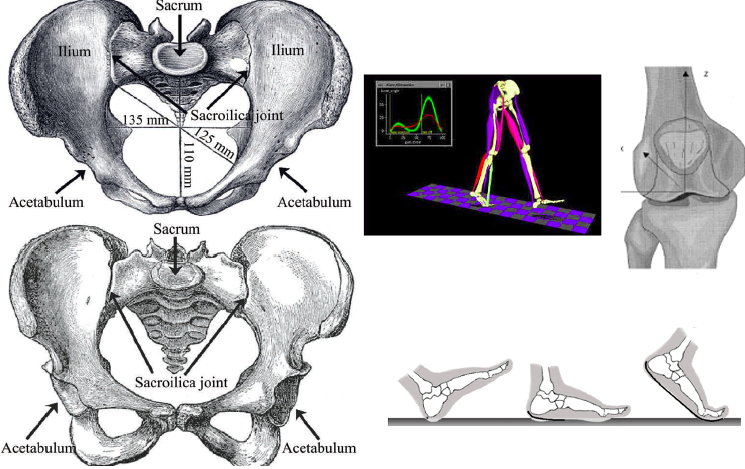
\includegraphics[height=7.0cm]{../images/ShortBiomechanics.png}}
    % \animategraphics[height=7cm,autoresume,autoplay]{0.8}{../images/ShortBiomechanics_}{0}{4}}
    \only<1>{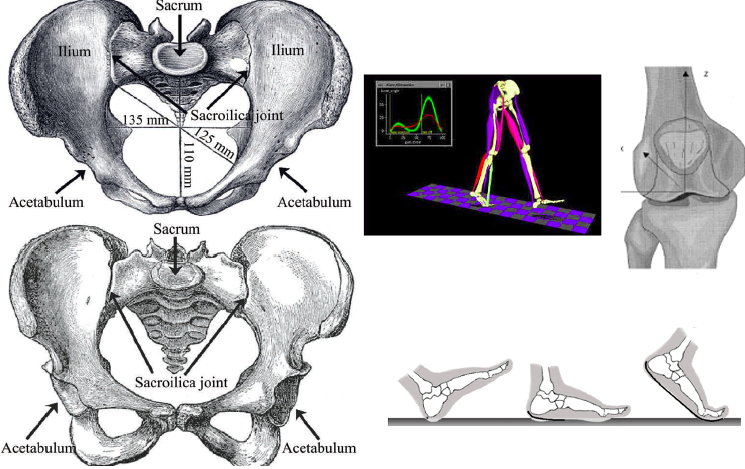
\includegraphics[height=7.0cm]{../images/ShortBiomechanics_0.png}}%
    \only<2>{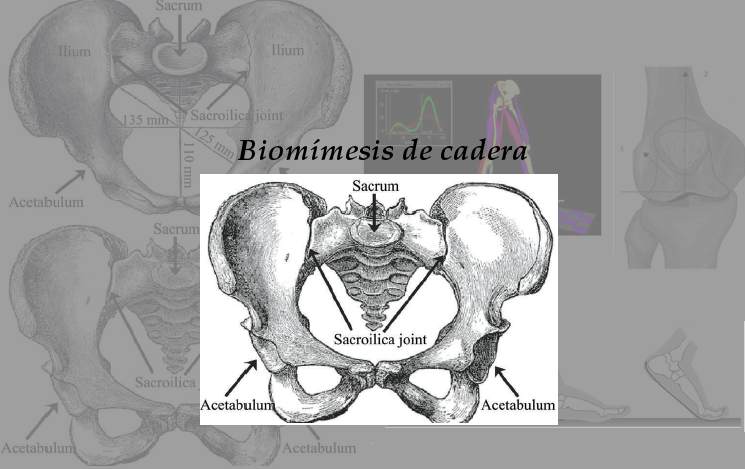
\includegraphics[height=7.0cm]{../images/ShortBiomechanics_1.png}}%
    \only<3>{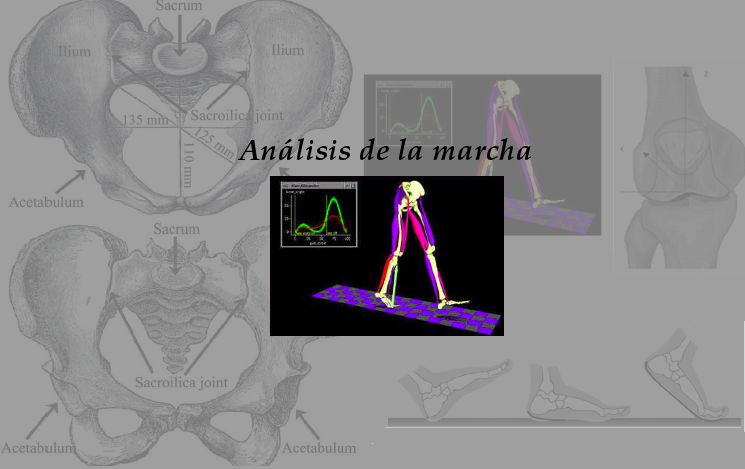
\includegraphics[height=7.0cm]{../images/ShortBiomechanics_2.png}}%
    \only<4>{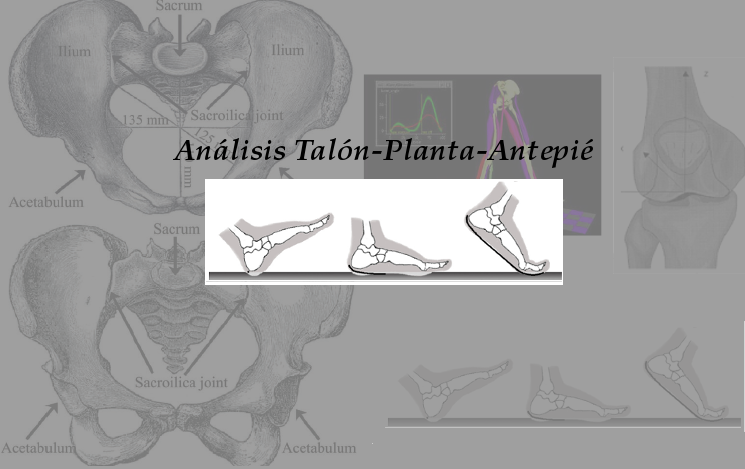
\includegraphics[height=7.0cm]{../images/ShortBiomechanics_3.png}}%
    \only<5>{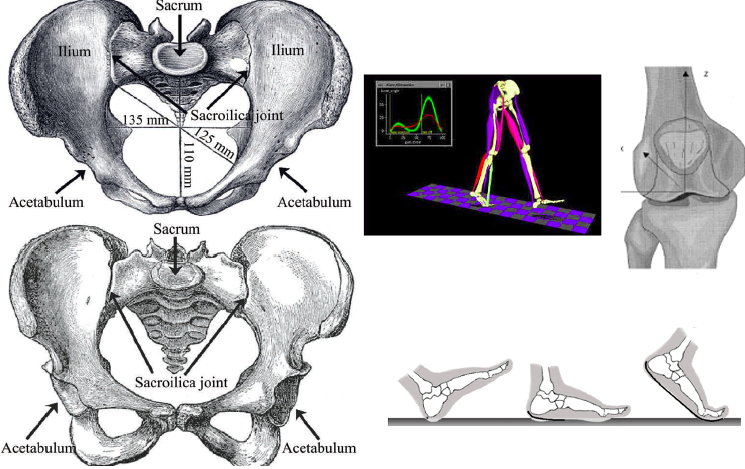
\includegraphics[height=7.0cm]{../images/ShortBiomechanics_4.png}}%
  }
  \hyperlink<1->{multidisciplinas<3>}{\beamerreturnbutton{Volver}}
\end{frame}